%!TEX root = ../doc.tex
\chapter{Fundamentals}
\label{sec:Fundamentals}
The following chapter describes methods and technologies that are used within this thesis.
\section{3D Cameras}
\label{sec:ToFCamera}
In the field of 3D mapping, two expressions often get mentioned: LiDaR sensors and ToF cameras. As the basic principle in both technologies relies on measuring the Time of Flight (ToF) and is in both cases Light-Detection and Ranging, both expressions are ambivalent.\\
A LiDaR sensor is often referred to work together with a moving laser, that scans its surroundings.\cite{Techradar_Lidar} The mechanical mounting of such a device is too bulky to be embedded in a modern smartphone, which is why solid-state LiDaR sensors are used. A solid-state LiDaR sensor projects a grid of laser dots onto the scene, as seen in image \ref{im:iPadLidar}. The time of flight for each dot is measured individually.
\begin{figure}[H]
    \centering
    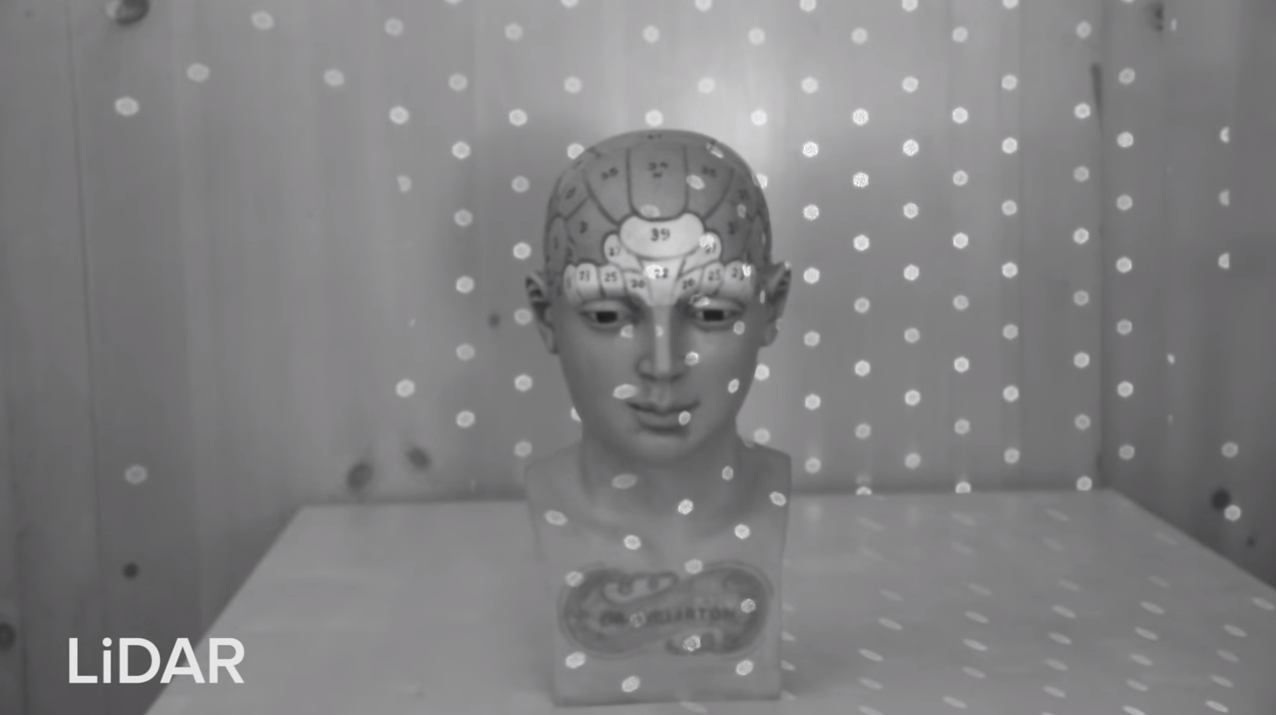
\includegraphics[width=1.0\textwidth]{images/ifixit_lidar.png}
    \caption{Projected dots from the LiDaR scanner of an Apple iPad Pro 2020, made visible with an infrared camera. Image source: iFixit.com}
    \label{im:iPadLidar}
\end{figure}
Another method for 3d mapping is, using one wide area infrared flash and measuring the time of flight on each individual sensor pixel. This approach in contrast is often referred to be a ToF camera. ToF cameras are used by different manufacturers of Android powered smart phones.\\
While the measurement principle in both technologies is the same, the LiDaR scanner generates a point cloud, while the ToF camera outputs a depth map image. With mathematical transformations, both outputs are equivalent. Another difference is that a ToF camera can double as a grayscale infrared camera, providing an image by itself. \\
The sensor used for this thesis follows the principle of a ToF camera. The measured radial distance from the sensor for each pixel allows the three dimensional reconstruction of the scene. 
\subsection{Radial information from ToF cameras}
\label{sec:RadialCorrection}
The used ToF camera provides the measured distance from the sensor to the filmed object for each pixel, generating a depht map. Because of the radial measurement, flat surfaces appear warped. The distortion follows a curve which can be corrected by knowing the cosine of the angle $\alpha$ for each pixel.
\begin{figure}[H]
    \centering
    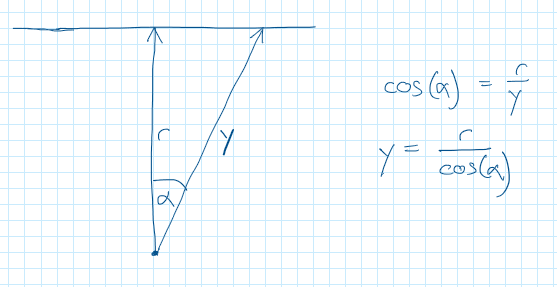
\includegraphics[width=0.5\textwidth]{images/dummy_radial_angle.png}
    \caption{Geometrics of the radial measurement and its correction.}
    \label{im:RadialCorrection}
\end{figure}
With the angle of the individual pixels being unknown, a map of cosine $\alpha$ is generated by taking an image of a flat surface.
\section{Mathematics for Rotation and Translation}
\label{sec:LinAlgRotation}
Augmented reality relies on having accurate positional and angular information to estimate the required size and warp of a virtual object projected into the real world. A MEMS module containing a gyroscope and an accelerometer provides rotation and acceleration information to the system to assist the positional tracking.
\subsection{Euler Rotations and Linear Algebra}
A common way to calculate rotations and translations are matrix-vector multiplications. The standard matrices for rotating with the angle $\phi$ around $X$, $Y$ and $Z$ are shown in the following:
\begin{equation*}
    A_{rot,X} =
    \begin{bmatrix}
        1 & 0        & 0         \\
        0 & cos \phi & -sin \phi \\
        0 & sin \phi & cos \phi
    \end{bmatrix}
    \quad
    A_{rot,Y} =
    \begin{bmatrix}
        cos \phi  & 0 & sin \phi \\
        0         & 1 & 0        \\
        -sin \phi & 0 & cos \phi
    \end{bmatrix}
    \quad
    A_{rot,Z} =
    \begin{bmatrix}
        cos \phi  & sin \phi & 0 \\
        -sin \phi & cos \phi & 0 \\
        0         & 0        & 1
    \end{bmatrix}
\end{equation*}
A combination of the three matrices leads to a rotation matrix with a rotation axis that is not strictly bound to $X$, $Y$, or $Z$. Matrix multiplication is not commutative, so the order of the multiplications matters. In the following example, the vector gets rotated first around $X$, then $Y$, and around $Z$ in the end. This chain of matrix operations is read from right to left in the equation.
\begin{equation*}
    A_{rot} =
    \begin{bmatrix}
        a_{0,0} & a_{0,1} & a_{0,2} \\
        a_{1,0} & a_{1,1} & a_{1,2} \\
        a_{2,0} & a_{2,1} & a_{2,2}
    \end{bmatrix}
    =A_{rot,Z} \cdot A_{rot,Y} \cdot A_{rot,X}
\end{equation*}
With this matrix, a three dimensional vector can be rotated at once around an arbitrary axis for the desired angle. Applying this transformation to each vertex of a virtual 3D object results in a rotation of the whole object around the origin $(0,0,0)$.\\
\begin{equation*}
    \begin{pmatrix}
        x' \\
        y' \\
        z'
    \end{pmatrix}
    =
    \begin{bmatrix}
        a_{0,0} & a_{0,1} & a_{0,2} \\
        a_{1,0} & a_{1,1} & a_{1,2} \\
        a_{2,0} & a_{2,1} & a_{2,2}
    \end{bmatrix}
    \cdot
    \begin{pmatrix}
        x \\
        y \\
        z
    \end{pmatrix}
\end{equation*}
To avoid using an inhomogenous linear system for moving an object, a fourth dimension is needed. By extending the vectors with a $1$ and using the fourth column in the matrix to alter $X$, $Y$ and $Z$, these vector entries can be moved without applying any rotation.
\begin{equation*}
    \begin{pmatrix}
        x+\Delta X \\
        y+\Delta Y \\
        z+\Delta Z \\
        1
    \end{pmatrix}
    =
    \begin{pmatrix}
        x' \\
        y' \\
        z' \\
        1
    \end{pmatrix}
    =
    \begin{bmatrix}
        1 & 0 & 0 & \Delta X \\
        0 & 1 & 0 & \Delta Y \\
        0 & 0 & 1 & \Delta Z \\
        0 & 0 & 0 & 1
    \end{bmatrix}
    \cdot
    \begin{pmatrix}
        x \\
        y \\
        z \\
        1
    \end{pmatrix}
\end{equation*}
To combine the rotation matrix with the translation matrix, the 3x3 rotation matrix gets placed top-left into the 4x4 unit matrix. Now, the rotation matrix also being a 4x4 matrix, rotations and translations can be chained up following the common laws of linear algebra. Chaining up translations and rotations allows moving the rotation axis for an object.
\begin{equation*}
    \begin{pmatrix}
        x' \\
        y' \\
        z' \\
        1
    \end{pmatrix}
    =
    \begin{bmatrix}
        a_{0,0} & a_{0,1} & a_{0,2} & 0 \\
        a_{1,0} & a_{1,1} & a_{1,2} & 0 \\
        a_{2,0} & a_{2,1} & a_{2,2} & 0 \\
        0       & 0       & 0       & 1
    \end{bmatrix}
    \cdot
    \begin{pmatrix}
        x \\
        y \\
        z \\
        1
    \end{pmatrix}
\end{equation*}
The dependency on the order of the rotations poses a problem visualized in image \ref{im:EulerRotation}: The values returned by a gyroscope would need to be applied all at once and not one after another.
\begin{figure}[H]
    \centering
    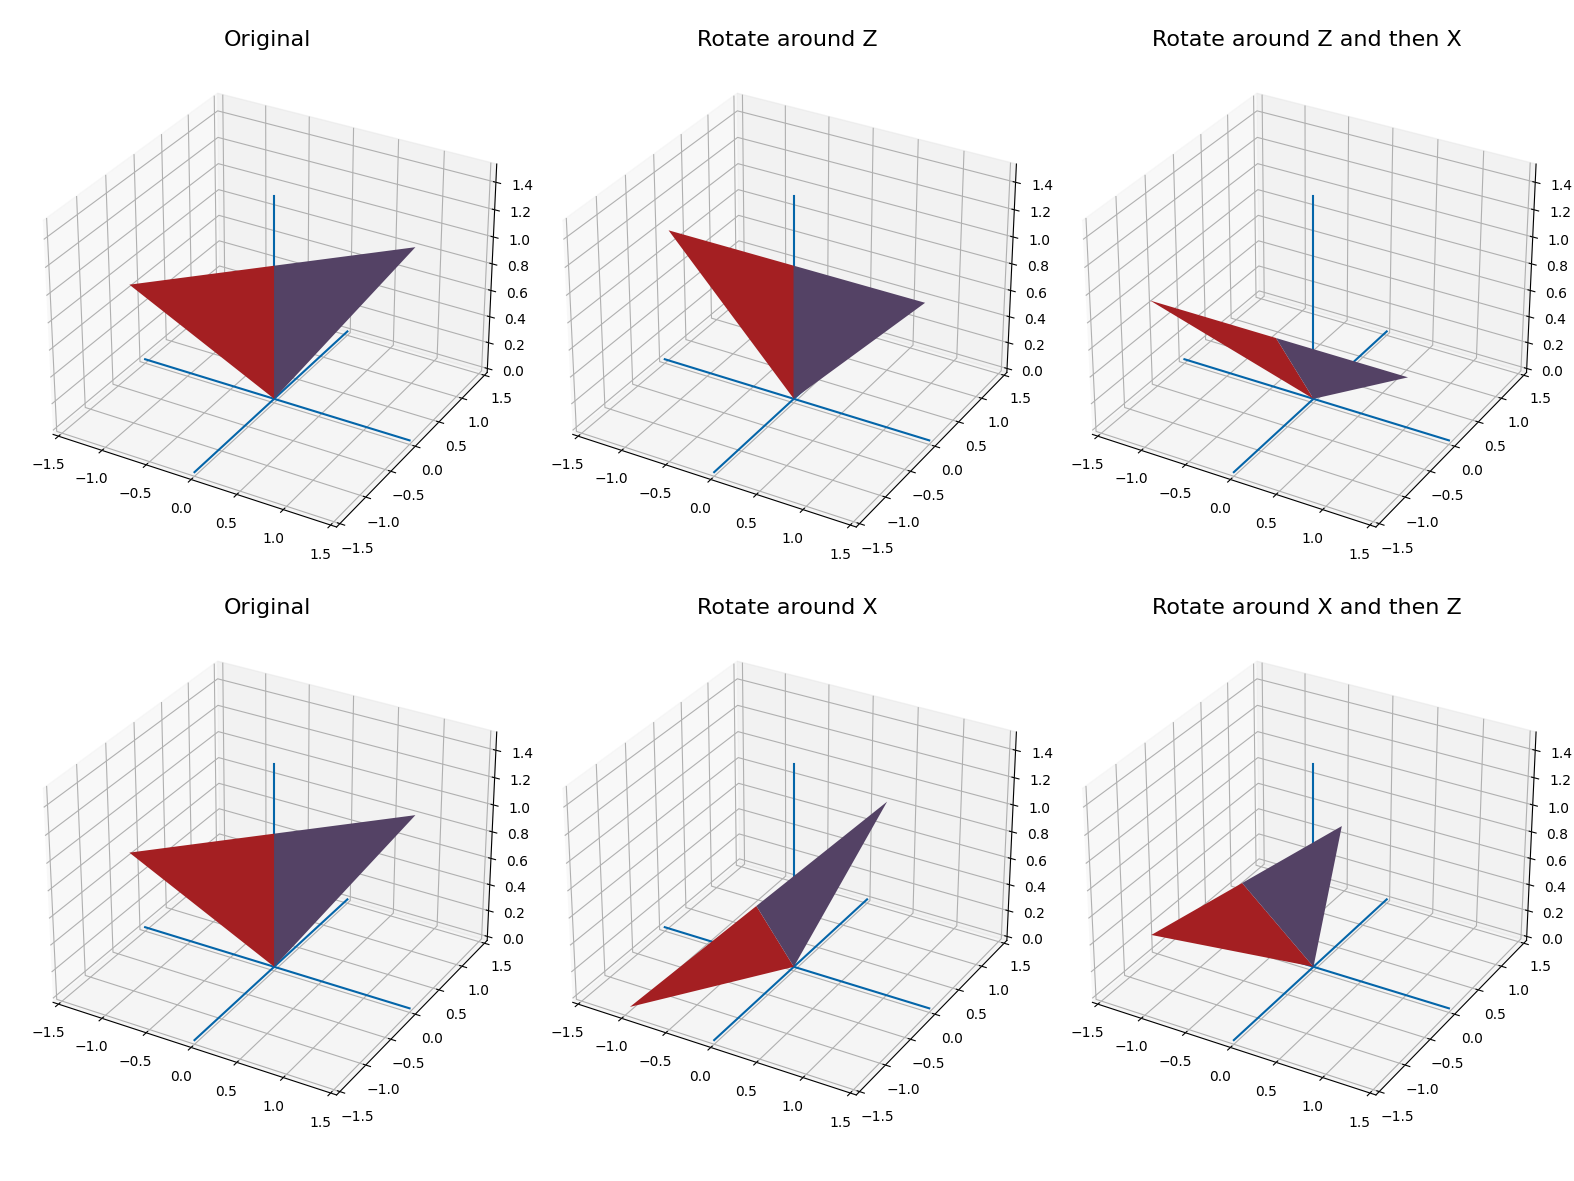
\includegraphics[width=1.0\textwidth]{images/euler_rotation.png}
    \caption{Euler rotations are dependent on the order of the individual rotations. Rotating around X and then Z results in a different outcome, than first rotating around Z and then X.}
    \label{im:EulerRotation}
\end{figure}
\subsection{Standard Vulkan Coordinate System}
In Vulkan, every vertex coordinate of a 3D rendered object gets mapped to the nearest pixel in the viewport window. This vertex mapping is done in multiple steps from "view coordinates" via "clip coordinates" towards "normalized device coordinates" to the "pixel coordinates".\\
A 3D object is a cloud of vertex coordinates described by a list three-dimensional vectors $\overrightarrow{v_{v}} = (x_{v},y_{v},z_{v})$ (the subscript $v$ denotes the "view coordinates"). These coordinates usually do not contain data regarding the whole object's scale, position, and rotation in 3D space - this information is added with matrices in the shader step.\\
Vulkan expects the output of the shader step to be in clip coordinates. Clip coordinates are four-dimensional vectors $\overrightarrow{v_{c}} = (x_{c},y_{c},z_{c},w_{c})$ (the subscript $c$ denotes the "clip coordinates") and the result of a matrix multiplication operation.\\
\begin{equation*}
    \overrightarrow{v_{c}} = A \cdot  \overrightarrow{v_{v}}
\end{equation*}
\begin{equation*}
    \begin{pmatrix}
        x_{c} \\
        y_{c} \\
        z_{c} \\
        w_{c}
    \end{pmatrix}
    =
    \begin{bmatrix}
        a_{0,0} & a_{0,1} & a_{M 0,2} & a_{0,3} \\
        a_{1,0} & a_{1,1} & a_{M 1,2} & a_{1,3} \\
        a_{2,0} & a_{2,1} & a_{M 2,2} & a_{2,3} \\
        a_{3,0} & a_{3,1} & a_{M 3,2} & a_{3,3}
    \end{bmatrix}
    \cdot
    \begin{pmatrix}
        x_{v} \\
        y_{v} \\
        z_{v} \\
        1
    \end{pmatrix}
\end{equation*}
Generally, three combined matrix multiplications describe how a 3D object is rendered – the model matrix, the view matrix, and an added projection matrix. The model matrix ($A_{Model}$) defines the scale, rotation and position of the 3D object and is a standard 4x4 matrix as explained in section \ref{sec:LinAlgRotation}.\\
The view matrix ($A_{View}$) is also is a rotation and translation matrix, but describes the position and direction of the viewport camera (or eye). Rotating the camera rotates the rendered virtual space, which indirectly moves and turns the models in the viewport. The linmath-library offers the "4x4\_look\_at" function that calculates the view matrix based on camera position, a viewing angle, and the information regarding the "upwards" direction.\\
The projection matrix ($A_{Projection}$)  is not a rotation and translation matrix besides the model and the view matrix. As its name suggests, the projection matrix reduces the vertex' 3d coordinates to the viewport plane by projecting them onto a virtual screen. By taking a field of view angle, the projection matrix allows camera distortion. The linmath-library offers the "4x4\_perspective" function that calculates the projection matrix based on a given field of view angle
Within the vertex shader, these three matrices are chained to perform the desired transformation.
\begin{equation*}
    A = A_{Projection} \cdot A_{View} \cdot A_{Model}
\end{equation*}
By division of the clip coordinate components $x_{c}$, $y_{c}$ and $z_{c}$ with $w_{c}$, Vulkan itself calculates the normalized device coordinates $\overrightarrow{v_{NDC}} = (x_{NDC}, y_{NDC}, z_{NDC})$.
\begin{equation*}
    \begin{pmatrix}
        x_{NDC} \\
        y_{NDC} \\
        z_{NDC} \\
    \end{pmatrix}
    =
    \begin{pmatrix}
        \frac{x_{c}}{w_{c}} \\
        \frac{y_{c}}{w_{c}} \\
        \frac{z_{c}}{w_{c}} \\
    \end{pmatrix}
\end{equation*}
The transformation to the pixel coordinates are also done by Vulkan without requiring any action by the developer. The only noticable detail is the alignment of the normalized device coordinates. On the viewport surface, the point $(0 / 0)$ is located in the center. Top left is $(-1 / -1)$, top right is $(1 / -1)$, bottom left is $(-1 / 1)$ and bottom right is $(1 / 1)$.

\subsection{Rotation with Quaternions}
\label{sec:RotationQuaternion}
Quaternions - also known as "Hamilton Numbers" - are the four dimensional equivalent to complex numbers. The theory of quaternions is vast, only the parts needed in this thesis are explained in this section. Analogue to complex numbers, quaternions also consist of a real part, but add three imaginary parts $\textbf{i}$, $\textbf{j}$ and $\textbf{k}$. Most often, quaternions get represented in the form $a+b\textbf{i}+c\textbf{j}+d\textbf{k}$ or a four dimensional vector $(a, b, c, d)$.\\
The relations of the different imaginary parts in a quaternion are defined as following: $\textbf{i}^{2}=\textbf{j}^{2}=\textbf{k}^{2}=\textbf{ijk}=-1$, $\textbf{ij}=\textbf{k}, \textbf{jk}=\textbf{j}, \textbf{ki}=\textbf{j}$, and  $\textbf{ji}=-\textbf{k}, \textbf{kj}=-\textbf{i}, \textbf{ik}=-\textbf{j}$. These definitions cause the quaternion multiplication (or Hamilton Product) to be non-commutative. The following equation shows how the Hamilton Product is calculated:
\begin{equation*}
    (a_{1}+b_{1}\textbf{i}+c_{1}\textbf{j}+d_{1}\textbf{k})(a_{2}+b_{2}\textbf{i}+c_{2}\textbf{j}+d_{2}\textbf{k})
    =
    \begin{pmatrix}
          & a_1a_2 &  & - b_1b_2 &  & - c_1c_2 &  & - d_1d_2             \\
        ( & a_1b_2 &  & + b_1a_2 &  & + c_1d_2 &  & - d_1c_2) \textbf{i} \\
        ( & a_1c_2 &  & - b_1d_2 &  & + c_1a_2 &  & + d_1b_2) \textbf{j} \\
        ( & a_1d_2 &  & + b_1c_2 &  & - c_1b_2 &  & + d_1a_2) \textbf{k}
    \end{pmatrix}
\end{equation*}
The neutral element of the quaternion multiplication is:
\begin{equation*}
    \begin{pmatrix}
        1           \\
        0\textbf{i} \\
        0\textbf{j} \\
        0\textbf{k}
    \end{pmatrix}
\end{equation*}
A plain three-dimensional vector is written in quaternions by only using the imaginary components.
\begin{equation*}
    \begin{pmatrix}
        x \\
        y \\
        z \\
    \end{pmatrix}
    =
    \begin{pmatrix}
        0           \\
        x\textbf{i} \\
        y\textbf{j} \\
        z\textbf{k}
    \end{pmatrix}
\end{equation*}
According to Euler's rotation theorem, providing a certain angle $\theta$ and a rotation axis $\vec{v_{r}}$, allows describing any rotation in three-dimensional space.
These values - the angle and the axis - are embedded within the rotation quaternion. In addition, the rotation quaternion is required to have the norm being equal one. Such a rotation quaternion is sometimes named a unit quaternion or a versor.
\begin{equation*}
    \vec{v}_{r} =
    \begin{pmatrix}
        x \\
        y \\
        z \\
    \end{pmatrix}
    \quad ; \quad
    \vec{v}_{r,norm} =
    \begin{pmatrix}
        \frac{x}{\lVert v_{r} \rVert} \\
        \frac{y}{\lVert v_{r} \rVert} \\
        \frac{z}{\lVert v_{r} \rVert}
    \end{pmatrix} =
    \begin{pmatrix}
        x_{norm} \\
        y_{norm} \\
        z_{norm}
    \end{pmatrix}
    \quad ; \quad
    Q_{rot}=
    \begin{pmatrix}
        \cos (\frac{\theta}{2} )                 \\
        x_{norm}\sin(\frac{\theta}{2})\textbf{i} \\
        y_{norm}\sin(\frac{\theta}{2})\textbf{j} \\
        z_{norm}\sin(\frac{\theta}{2})\textbf{k}
    \end{pmatrix}
    \quad ; \quad
    \lVert Q_{Rot} \rVert = 1
\end{equation*}
To apply this rotation quaternion $Q_{rot}$ to a vector $\vec{v}$, it needs to be conjugated and calculated from the front and from the back as shown in the following. Conjugation of a unit quaternion is done by flipping the sign in each imaginary part. Vector $\vec{u}$ is the rotated vector $\vec{v}$.
\begin{equation*}
    \vec{v} =
    \begin{pmatrix}
        a \\
        b \\
        c \\
    \end{pmatrix}
    =
    \begin{pmatrix}
        0           \\
        a\textbf{i} \\
        b\textbf{j} \\
        c\textbf{k}
    \end{pmatrix}
    \quad ; \quad
    \vec{u} = Q_{rot}\vec{v}Q_{rot}^{-1}=\begin{pmatrix}
        \cos (\frac{\theta}{2} )                 \\
        x_{norm}\sin(\frac{\theta}{2})\textbf{i} \\
        y_{norm}\sin(\frac{\theta}{2})\textbf{j} \\
        z_{norm}\sin(\frac{\theta}{2})\textbf{k}
    \end{pmatrix}
    \begin{pmatrix}
        0           \\
        a\textbf{i} \\
        b\textbf{j} \\
        c\textbf{k}
    \end{pmatrix}
    \begin{pmatrix}
        \cos (\frac{\theta}{2} )                  \\
        -x_{norm}\sin(\frac{\theta}{2})\textbf{i} \\
        -y_{norm}\sin(\frac{\theta}{2})\textbf{j} \\
        -z_{norm}\sin(\frac{\theta}{2})\textbf{k}
    \end{pmatrix}
\end{equation*}
By converting a rotation quaternion to a rotation matrix, the gap to Vulkan can be bridged. This formula only applies to true rotation quaternions, therefore the norm needs to be equal to one. 
\begin{equation*}
    Q_{Rot}=    \begin{pmatrix}
        a           \\
        b\textbf{i} \\
        c\textbf{j} \\
        d\textbf{k}
    \end{pmatrix}
    \quad ; \quad
    \lVert Q_{Rot} \rVert = 1
    \quad ; \quad
    A_{Rot}
    =
    \begin{bmatrix}
        1-2(c^{2}+d^{2}) & 2(bc-ad) & 2(bd+ac) \\
        2(bc+ad) & 1-2(b^{2}+d^{2}) & 2(cd-ab) \\
        2(bd-ac) & 2(cd+ab) & 1-2(b^{2}+c^{2})
    \end{bmatrix}
\end{equation*}
The basic quaternion operations - like the multiplication - are included in the linmath-library. The linmath-library represents a quaternion as a four-dimensional float-vector in the ordering $(b, c, d, a)$ - the real part being the last element.\\
\section{Motion detection by camera and depth information}
Turning or moving the camera head influences the image of an object differently, based on its distance to the camera. The position of a single point within the image depends on the coordinates of the point in the real space, as shown in image \ref{im:opticalAxis}. The optical axis matches with the $x$ axis while the sensor plane lies in the $YZ$ plane.
\begin{figure}[H]
    \centering
    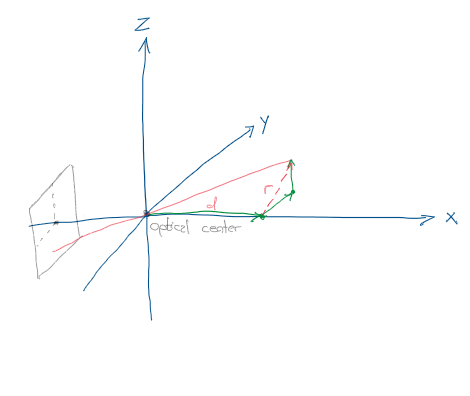
\includegraphics[width=0.5\textwidth]{images/dummy_optical_axis.png}
    \caption{Projection of a point in space to the image sensor.}
    \label{im:opticalAxis}
\end{figure}
\subsection{Singular Value Decomposition (SVD)}
\label{sec:SVD}
The singular value decomposition is a linear algebra method that allows finding the optimal rotation matrix between two matching point clouds. Adding additional algebraic steps makes it possible to find the optimal translation vector in addition.\cite{SVD_ETH}
For demonstration purposes, the recipe is carried out in a 3D example in section \ref{sec:ToFPosition_SVD} in the Implementation chapter.\\
The SVD decomposes any given matrix $M$ of the dimension $n\times m$ into three matrices $U$ of dimension $n\times n$, $\Sigma$ of dimension $n\times m$, and $V$ of dimension $m\times m$.\cite{SVD_MIT} If $M$ is real, $U$ and $V$ are guaranteed to be orthogonal, while $\Sigma$ is a diagonal matrix. The matrices fulfill the following equation: 
\begin{equation*}
    M= U\Sigma V^{T}
\end{equation*}
The individual matrices generated by the SVD act als two rotations and one distortion. As visible in image \ref{im:SVD}, the unit circle $\vec{x}$ first gets rotated by $V^{T}$ that the distortion is in the directions of the coordinate system. After applying the distortion $\Sigma$ to the rotated circle $\vec{y}_{1}$, the intermediate ellipse $\vec{y}_{2}$ gets rotated and mirrored to match $\vec{y}$.
\begin{figure}[h]
    \centering
    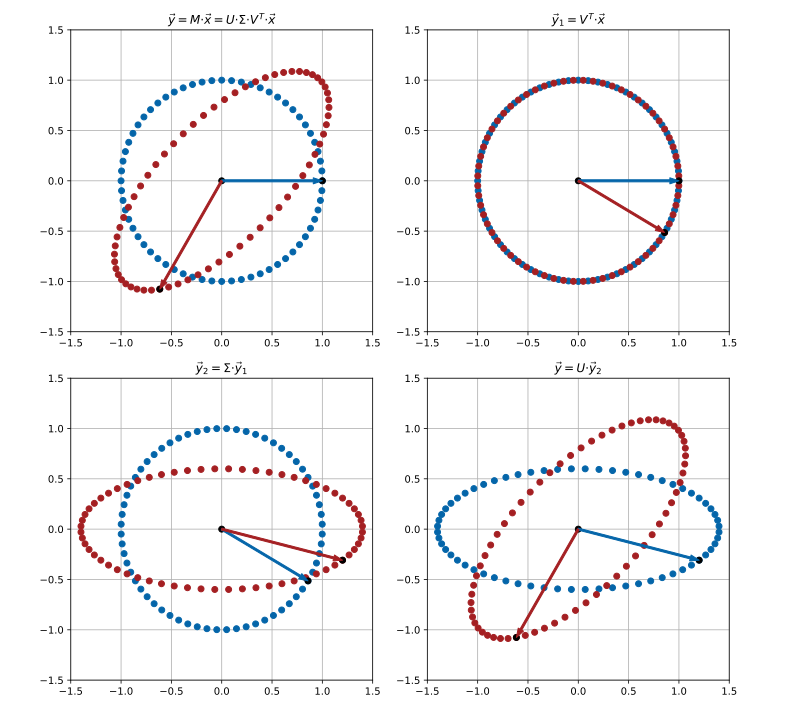
\includegraphics[width=0.7\textwidth]{images/SVD}
    \caption{Singular Value Decomposition in 2D shown in the individual stages. Blue is before and red is after the applied transformation.}
    \label{im:SVD}
\end{figure}
The following recipe\cite{SVD_MIT} shows how to find the matrices of the singular value decomposition. The matrix $M$ that is used in visualization \ref{im:SVD} gets decomposed.
\begin{equation*}
    M= 
    \begin{bmatrix}
        0.6 & 0.9  \\
        1.1 & 0.2
    \end{bmatrix}  
\end{equation*}
In order to find $U$, the eigenvectors $\vec{v}_{1}$ and $\vec{v}_{2}$ of $MM^{T}$ have to be calculated, that are directly filled in:
\begin{equation*}
    MM^{T}= 
    \begin{bmatrix}
        1.17 & 0.84  \\
        0.84 & 1.25
    \end{bmatrix}  \quad
    \vec{v}_{1} =
    \begin{pmatrix}
        -0.6901 \\
        -0.7237
    \end{pmatrix}\quad
    \vec{v}_{2} =
    \begin{pmatrix}
        -0.7237 \\
        0.6901
    \end{pmatrix}\quad
    U= 
    \begin{bmatrix}
        -0.6901 & -0.7237  \\
        -0.7237 & 0.6901
    \end{bmatrix}
\end{equation*}
Similarly to $U$, the eigenvectors of $M^{T}M$ deliver $V$:
\begin{equation*}
    M^{T}M= 
    \begin{bmatrix}
        1.57 & 0.76  \\
        0.76 & 0.85
    \end{bmatrix}  \quad
    \vec{v}_{1} =
    \begin{pmatrix}
        -0.8450 \\
        0.5347
    \end{pmatrix}\quad
    \vec{v}_{2} =
    \begin{pmatrix}
        -0.5347 \\
        -0.8450
    \end{pmatrix}\quad
    V= 
    \begin{bmatrix}
        -0.8450 & -0.5347  \\
        0.5347 & -0.8450
    \end{bmatrix}
\end{equation*}
Finally, the square-roots of the eigenvalues of either $M^{T}M$ or $MM^{T}$ are the diagonal values of $\Sigma$:
\begin{equation*}
    \Sigma= 
    \begin{bmatrix}
        1.4321 & 0  \\
        0 & 0.6075
    \end{bmatrix}
\end{equation*}
\section{Camera Calibration}
\label{sec:FundCamCalibration}
An uncalibrated camera image often has lens distortion, warping a rectangle into a pillow or barrel shape and making areas appear closer in certain parts of the image. These distortions are named radial and tangential distortion and are induced by the camera lens.\\
According to OpenCV \cite{openCVCamCalib}, radial distiortion can be modeled as:
\begin{equation*}
x_{distorted} = x(1+k_{1}r^{2}+k_{2}r^{4}+k_{3}r^{6})\qquad
y_{distorted} = y(1+k_{1}r^{2}+k_{2}r^{4}+k_{3}r^{6})
\end{equation*}
Tangential distortion is modeled as\cite{openCVCamCalib}:
\begin{equation*}
    x_{distorted} = x+(2p_{1}xy+p_{2}(r^{2}+2x^{2}))\qquad
    y_{distorted} = y+(p_{1}(r^{2}+2y^{2})+2p_{2}xy)
\end{equation*}
In these equations, $r$ is the euclidian distance between the distorted image point and the distortion center.\cite{openCVCamCalib}\\
\begin{equation*}
    r=\sqrt{(x_{distorted}-x_{center})^{2}+(y_{distorted}-y_{center})^{2}}
\end{equation*}
Therefore, for the lens distortions, the five coefficients $k_{1}$, $k_{2}$, $k_{3}$, $p_{1}$ and $p_{2}$ are needed. In addition, the effect of the focal length $f$ and the optical center $c$ get expressed as a 3x3 matrix.\cite{openCVCamCalib}
\begin{equation*}
    A_{Camera}=
    \begin{bmatrix}
        f_{x} & 0 & c_{x} \\
        0 & f_{y} & c_{y} \\
        0 & 0 & 1
    \end{bmatrix}
\end{equation*}
OpenCV itself provides a script which estimates these values based on multiple photographs of chess boards. Applying these corrections leads to a smaller image as parts near the border get cut off.
\begin{figure}[H]
    \centering
    \begin{minipage}[b]{0.45\textwidth}
      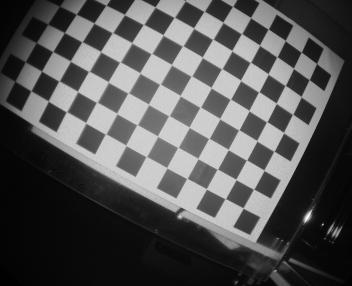
\includegraphics[scale=0.70]{images/camcalib_source.jpg}
      \caption{Before correction}
      \label{fig:camCalibBefore} 
    \end{minipage} % Hier darf keine Leerzeile zwischen den beiden Minipages liegen!
    \begin{minipage}[b]{0.45\textwidth}
      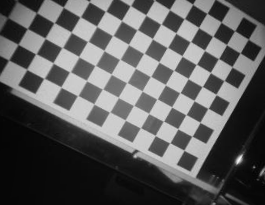
\includegraphics[scale=0.70]{images/camcalib_result.png} 
      \caption{After correction}
      \label{fig:camCalibAfter} 
    \end{minipage}
    \caption{Camera correction demonstrated at the grayscale image of the ToF camera.}
    \label{fig.camCalib}
  \end{figure}
The implementation in CUDA is done by storing the pixel coordinates of the uncorrected image for each pixel in the corrected image. This data is loaded into a CUDA allocated memory area and allows mapping the coordinates for the correction without complex caluclations as visualized in image \ref{im:CudaCamCalib}.
\begin{figure}[H]
    \centering
    
\includegraphics[width=1.0\textwidth]{images/todo.png}
    \caption{Storing the final calibration values into an array keeps the implementation in CUDA simple.}
    \label{im:CudaCamCalib}
\end{figure}